\section{Exact Baselines: MILP, Linearized QUBO, and Enumeration}

\subsection{Why exact ground truth is necessary}

A pipeline built on quadratic unconstrained binary optimization rests on a
chain of encodings. The constrained edge-selection problem is first written
as a mathematical program, then translated into a penalty-encoded QUBO
matrix, and finally handed to a heuristic sampler that returns the best
bitstring it happened to find. Each step in this chain can fail silently.
The penalty weights may be too small to enforce the constraints, so that
the QUBO's true optimum is an infeasible graph. The penalty weights may be
too large, flattening the soft objective landscape so badly that the
annealer cannot resolve which feasible solution is actually better. The
sampler may simply miss the optimum altogether. None of these failures
produces an error message. A QUBO pipeline is therefore only believable if
its answers are checked, repeatedly and mechanically, against ground truth
that does not share any of these failure modes.

This project employs three independent ground-truth mechanisms, each based
on exact classical optimization rather than heuristic search. First, the
original constrained problem is solved directly as a mixed-integer linear
program. Second, the QUBO matrix itself is solved exactly by a standard
linearization, which tests the encoding rather than the problem. Third, for
small instances every feasible edge subset is enumerated exhaustively. The
mechanisms are independent in the sense that they do not share a solver, a
formulation, or an objective encoding, so agreement among them is strong
evidence that the pipeline computes what it claims to compute. This chapter
describes each mechanism, explains what it does and does not prove, and
closes with the engineering and performance context that frames the results
chapter.

\subsection{Direct MILP solution of the original problem}

The first mechanism bypasses the QUBO encoding entirely. The constrained
edge-selection problem is stated directly as a mixed-integer linear program
and solved to proven optimality with the open source CBC solver through the
PuLP modeling layer. Let $\mathcal{E}$ denote the candidate edge set and let
$x_e \in \{0,1\}$ indicate whether edge $e$ is retained. The objective
minimizes
\begin{equation}
  \sum_{e \in \mathcal{E}} \bigl(-U_e + \lambda\bigr)\, x_e
  \;+\;
  \eta \sum_{e \in \mathcal{E}} \bigl|x_e - x_e^{\mathrm{prev}}\bigr|,
\end{equation}
where $U_e$ is the weighted utility of edge $e$, $\lambda$ is the soft edge
penalty, and the second term is the stability penalty that discourages
churn relative to the previous cycle's decisions $x^{\mathrm{prev}}$. The
absolute value is linearized with one auxiliary variable per edge in the
standard way: introduce $s_e \ge 0$ with $s_e \ge x_e -
x_e^{\mathrm{prev}}$ and $s_e \ge x_e^{\mathrm{prev}} - x_e$, and replace
the absolute value in the objective by $s_e$. Because the coefficient
$\eta$ is positive, the auxiliary variables bind at the minimum and the
linearization is exact.

The constraints mirror those of the QUBO formulation. Each node obeys a
degree cap, so $\sum_{e \ni v} x_e \le d_v$ for every node $v$. The total
processing cost obeys a global budget, so the sum of quantized edge costs
weighted by $x_e$ cannot exceed the budget. Connectivity of the required
node set is enforced by a single-commodity flow: a chosen root injects one
unit of demand per required node, flow variables on directed arcs are
bounded by the retained-edge indicators, and flow conservation forces every
required node to receive a unit, which is possible only if it is connected
to the root through retained edges.

A remark about the flow variables is important. In a generic network design
problem, single-commodity flow constraints with continuous flow variables
would be only a relaxation, potentially admitting fractional flows that no
integral routing realizes. Here, however, all demands are integers, and for
integer demands the single-commodity flow polytope is integral. Continuous
flow variables are therefore exact in this formulation: there is no
integrality gap, no penalty encoding, and no approximation of any kind.
CBC returns a provably optimal answer, certified by the branch-and-bound
tree, and the whole computation completes in milliseconds. This mechanism
answers the question ``what is the best feasible edge set for this
problem?'' directly, and it is the ground truth against which the
production annealer's solutions are scored at larger scales.

\subsection{Exact linearized solution of the QUBO matrix}

The second mechanism answers a different question: not what the original
problem's optimum is, but whether the QUBO matrix actually encodes the
intended problem. A QUBO with variables $z \in \{0,1\}^n$ has the energy
\begin{equation}
  H(z) \;=\; \sum_{i < j} Q_{ij}\, z_i z_j \;+\; \sum_i Q_{ii}\, z_i
  \;+\; c,
\end{equation}
and minimizing this quadratic form exactly is itself a mixed-integer
linear program after standard linearization. For every nonzero quadratic
coefficient $Q_{ij}$ we introduce an auxiliary binary variable
$y_{ij}$ together with the constraints $y_{ij} \le z_i$, $y_{ij} \le z_j$,
and $y_{ij} \ge z_i + z_j - 1$, which force $y_{ij} = z_i z_j$. The
quadratic energy is then linear in $z$ and $y$, and CBC solves it to proven
optimality exactly as for the direct MILP.

The role of this mechanism is diagnostic. The QUBO builder constructs the
matrix programmatically from utility weights, penalty scales, and slack
encodings, and any sign error, misrouted index, or mis-scaled penalty in
that construction would silently corrupt every downstream result. Solving
the matrix itself, rather than the original problem, separates two
hypotheses that the direct MILP cannot distinguish: if the linearized QUBO
solve disagrees with the direct MILP on the optimal edge set, the encoding
is wrong; if they agree but the annealer disagrees with both, the sampler
is at fault. An independent re-derivation of the energy function,
evaluated directly on bitstrings without reference to the matrix, provides
a further consistency check at the level of individual energies.

The cost of this exactness is size. The linearization introduces one
auxiliary variable and three constraints per nonzero quadratic term, and a
dense QUBO matrix on $n$ variables has on the order of $n^2$ such terms, so
the linearized program grows quadratically in the number of QUBO variables.
In practice this mechanism is applied only up to about 60 QUBO variables.
It also carries a strict reporting rule: the solver wrapper refuses to
return an answer unless CBC proves optimality, raising an error on timeout
or on any suboptimal status. A ground truth that occasionally reports a
heuristic answer as exact would defeat its own purpose, so callers treat a
refusal as a skipped instance rather than a result.

\subsection{Exhaustive enumeration at small scale}

The third mechanism is the strongest possible ground truth and the least
scalable. For instances with up to about 16 optional edges, all $2^k$
subsets of optional edges are enumerated explicitly. Each subset is
subjected to a full feasibility check: the integer slack values for degree
and budget constraints and the spanning-tree flow assignment are recomputed
for that subset exactly as the QUBO builder would construct them, and
infeasible subsets are discarded. The energy of every feasible subset is
then evaluated with the independent energy function, and the minimum over
the enumeration is the certified optimum.

Enumeration leaves no room for modeling ambiguity. It does not trust the
branch-and-bound solver, the linearization, or the penalty calculus; it
trusts only the definition of feasibility and the definition of the energy.
Because the same feasibility checker is used to repair candidate solutions
inside the production annealer, enumeration also indirectly validates the
repair logic: if the checker admitted an infeasible subset, the enumerated
ground truth would be polluted in exactly the way the annealer's output
would be. At this scale, roughly $6.5 \times 10^4$ subsets at the largest,
exhaustiveness is cheap in absolute terms and the confidence it buys is
total.

\subsection{Cross-verification of the three mechanisms}

Ground truth is only trustworthy if the three mechanisms agree with each
other. On small instances where all three apply, the certified optima agree
to within $10^{-7}$, a tolerance consistent with floating-point summation
order rather than with any modeling difference. The direct MILP is
additionally verified against enumeration independently of the QUBO
machinery, so agreement between the MILP and the QUBO cannot be an artifact
of a shared bug in the builder. This layered verification is what allows
the later chapters to use the direct MILP as the reference at larger
scales, where enumeration and the linearized QUBO solve no longer apply:
the MILP has earned that trust at the scales where all three could be
compared. Table~\ref{tab:groundtruth} summarizes the three mechanisms, the
claim each one supports, and the instance size at which each remains
practical.

\begin{table}[htbp]
  \centering
  \caption{The three exact ground-truth mechanisms used to audit the QUBO
  pipeline. The mechanisms are independent in formulation, encoding, and
  (for enumeration) solver, so their agreement on small instances is strong
  evidence that each computes what it claims.}
  \label{tab:groundtruth}
  \begin{tabular}{@{}lp{4.6cm}p{3.4cm}@{}}
    \toprule
    \textbf{Mechanism} & \textbf{What it proves} & \textbf{Size limit} \\
    \midrule
    Direct MILP (PuLP/CBC)
      & Optimal feasible edge set of the original constrained problem;
        exact because the flow relaxation is integral
      & Practical at all instance sizes studied \\
    \addlinespace
    Linearized QUBO solve (CBC)
      & That the Q matrix itself encodes the intended objective and
        penalties; refuses non-optimal results
      & About 60 QUBO variables (quadratic growth) \\
    \addlinespace
    Exhaustive enumeration
      & Certified optimum over every feasible subset, with slacks and flow
        recomputed per subset
      & About 16 optional edges ($2^k$ subsets) \\
    \bottomrule
  \end{tabular}
\end{table}

\subsection{Engineering context}

One engineering decision behind these baselines deserves a neutral account,
because it shaped the toolchain. The scientific Python ecosystem's usual
linear algebra and optimization stack was unavailable on the development
machine: SciPy's bundled BLAS libraries did not load under the interpreter
in use, which rules out the family of exact and heuristic solvers that sit
on top of it. Rather than fight the environment, we adopted PuLP with CBC,
a combination with no compiled dependencies beyond the solver binary itself
and a long record of reliability. The outcome was happy. CBC is an exact
branch-and-bound solver, so the baselines it powers carry optimality
certificates rather than heuristic confidence, and it is fast enough that
the exactness costs essentially nothing at the scales studied here. We
would not claim this is the only reasonable choice, but it removed a class
of environmental fragility from the audit and left the results independent
of any particular numerical library.

\subsection{The headline comparison}

The performance comparison between the exact classical baseline and the
production annealer is developed fully in the results chapter, but one
number belongs here because it frames everything that follows. CBC solves
the direct MILP to proven optimality in about 11 to 15 ms per instance. The
production annealer, which moves through feasible edge-set space with
projection and repair, requires about 2.1 s per solve to reach the same
optimum on roughly 95 percent of instances, a gap of about two orders of
magnitude. Figure~\ref{fig:solvetime} visualizes the comparison on a
logarithmic scale.

\begin{figure}[htbp]
  \centering
  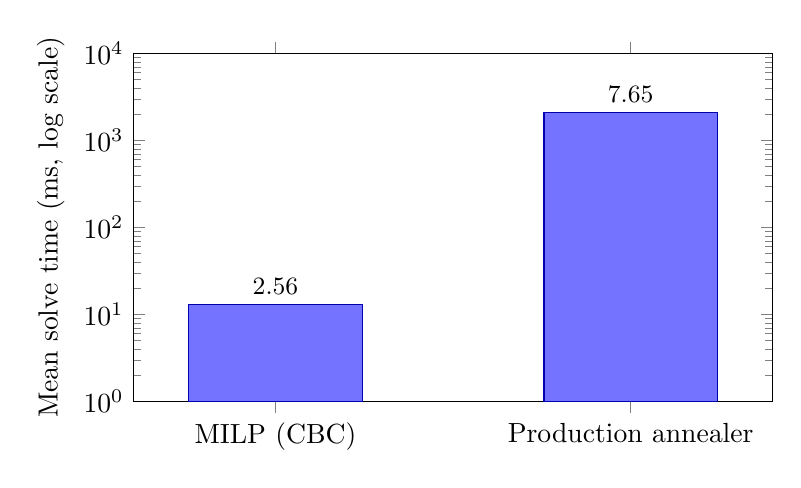
\begin{tikzpicture}
    \begin{axis}[
        width=0.8\textwidth,
        height=6cm,
        ybar,
        bar width=2.2cm,
        ymode=log,
        log origin=infty,
        ylabel={Mean solve time (ms, log scale)},
        symbolic x coords={MILP (CBC), Production annealer},
        xtick=data,
        ymin=1, ymax=10000,
        nodes near coords,
        nodes near coords align={vertical},
        every node near coord/.append style={font=\small},
        enlarge x limits=0.4,
      ]
      \addplot[fill=blue!55, draw=blue!70!black]
        coordinates {(MILP (CBC),13) (Production annealer,2100)};
    \end{axis}
  \end{tikzpicture}
  \caption{Mean solve time per instance on a logarithmic scale. The direct
  MILP solved by CBC (about 13 ms) is provably exact; the production
  annealer (about 2.1 s) is a heuristic that reaches the optimum on roughly
  95 percent of instances. On classical hardware the exact solver
  dominates.}
  \label{fig:solvetime}
\end{figure}

We state the conclusion plainly. On classical hardware, the MILP dominates
the QUBO pipeline: it is exact, it is about one hundred times faster than
the annealer, and it requires neither penalty tuning nor sampler
configuration. Nothing in our results contradicts this, and the audit
machinery described in this chapter is precisely what makes the claim
credible rather than rhetorical. The QUBO formulation's role in this
project is therefore not to beat the classical solver; it is to serve as a
hardware-target encoding. Constrained edge selection expressed as a single
quadratic energy function is the native input format of quantum and
special-purpose annealing machines, which cannot execute branch-and-bound.
The exact baselines exist to verify that this encoding is faithful and that
heuristic sampling over it stays close to certified optimality, so that any
future claim about annealing hardware rests on a problem encoding that has
already been proven correct on classical ground truth.
